%%% Local Variables:
%%% mode: latex
%%% TeX-master: "../doc"
%%% coding: utf-8
%%% End:
% !TEX TS-program = pdflatexmk
% !TEX encoding = UTF-8 Unicode
% !TEX root = ../doc.tex
\section{Vergleich LOD-Systeme}
Die verschiedenen \e{LOD}-Systeme, sowie ihre Vor- und Nachteile werden in \autoref{chap:differentLodApproaches} definiert. In diesem Schritt wird erläutert, welche Art \e{LOD}-System es bereits gibt und welches in dieser Arbeit entwickelt werden soll.

\subsection{Bestehende Systeme}
\label{chap:existingSolutions}

\e{Unity} sowie \e{Unreal} verfügen über umfangreiche \e{LOD}-Systeme. Eine Analyse dieser Systeme bildet somit die Grundlage für die Entwicklung eines neuen Systems.

\paragraph{Unreal}

\e{Unreal} verfügt sowohl über ein \e{DLOD}-System als auch über ein \e{HLOD}-System. Das \e{HLOD}-Tool zeichnet sich insbesondere dadurch aus, dass es die verschiedenen Artefakte automatisch generieren kann. Dies ermöglicht es, komplexe Strukturen direkt innerhalb von \e{Unreal} zu kombinieren \cite{unrealProxyLod}.
So können einige Faktoren angepasst werden, um die \e{LOD} den Anforderungen entsprechend zu gestalten. Das Ergebnis kann direkt in einer Vorschau überprüft werden, wie in Abbildung \ref{fig:unrealLODGeneration}. So wird es leicht gemacht, Feinjustierungen vorzunehmen.
Der Moment für die Levelwahl kann eingestellt werden. \e{Unreal} bietet eine automatische Option, so wie auch eine manuelle, wobei für jedes Level der Triggerpunkt gewählt werden kann.
\e{Unreal} lässt Benutzer den Triggerpunkt über die relative Grösse eines Modells zur Fenstergrösse einstellen. Dies hat zwei wesentliche Vorteile: Einerseits können so Modelle in verschiedenen Grössen verwendet werden, welche alle individuelle Triggerzeitpunkte haben. Andererseits ist diese Grösse einfach zu testen und benötigt somit für die Einstellung weniger manuellen Aufwand.
Der Zeitaufwand für die Integration des Systems in eine Applikation wird so signifikant reduziert und macht den Einsatz eines \e{LOD}-Systems attraktiver.

\begin{figure}[H]
  \centering
  \includegraphics[width=0.8\columnwidth]{vorgehen/Unreal-LOD.png}
  \caption{Automatische \e{LOD}-Generierungsansicht in \e{Unreal} \cite{unrealAutoLod}}
  \label{fig:unrealLODGeneration}
\end{figure}

\paragraph{Unity}

\e{Unity} verfügt über ein \e{DLOD}-System, welches es erlaubt \e{LOD}-Artefakte manuell zu definieren.
Innerhalb der \e{Unity} Community gibt es eine Bibliothek für das automatische Generieren von Artefakten, welche für \e{LOD} verwendet werden können \cite{unityMeshSimplification}.
Ansätze für ein \e{HLOD}-System sind vorhanden, wurden jedoch nicht offiziell in \e{Unity} integriert \cite{unityAutoLod}.

In Abbildung \ref{fig:unityDLODGroup} ist ersichtlich, wie innerhalb von Unity der Übergang zwischen zwei \e{LOD}-Artefakten konfiguriert werden kann. Hervorzuheben sind hier zum einen der \e{Fade Mode}, der das \e{Visual Popping} vermindert und zum anderen die Triggerpunkte, bei welchen das Level gewechselt werden soll.
Dies wird in \e{Unity} identisch zu \e{Unreal} gelöst, in dem der Triggerpunkt relativ zur Fenstergrösse festgelegt wird.

\begin{figure}[H]
  \centering
  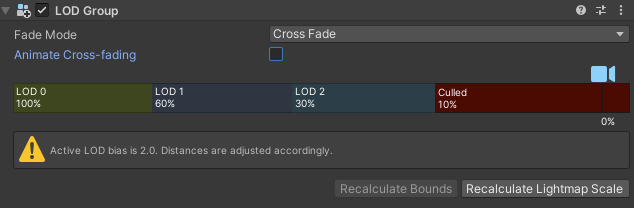
\includegraphics[width=0.8\columnwidth]{vorgehen/Unity-DLOD.png}
  \caption{'\e{LOD Group}'-Komponente in Unity für die Konfiguration der Übergänge zwischen \e{LOD}-Artefakten}
  \label{fig:unityDLODGroup}
\end{figure}

\subsection{Kriterien}

Die verschiedenen Ansätze unterscheiden sich in einigen Kriterien. Für den Einsatz in einer Web-Anwendung ist die Gewichtung der Kriterien anders als für Desktop-Anwendungen, Konsolenspiele oder dergleichen.
So hat die Dateigrösse der Modelle bei Web-Anwendungen einen grösseren Einfluss auf die gefühlte Performanz beim Endanwender. Insofern ist die Auswirkung der gewählten Strategie auf die Downloadgrösse ein wichtiges Kriterium.

\subsection{Vergleich Downloadgrösse}

Für diskrete \e{LOD} muss für jedes Level ein separates Modell geladen werden. Dies kann die Downloadgrösse gegebenenfalls merkbar erhöhen. Bei kontinuierlichen \e{LOD}-Systemen muss das Modell die Unterschiede zwischen verschiedenen Levels persistieren. Mit einem für kontinuierliche \e{LOD} ausgelegten Algorithmus kann der benötigte Speicher reduziert werden, indem beim \e{Edge Collapse} nicht auf einen neuen optimalen \e{Vertex} reduziert wird, sondern von den beiden bestehenden \e{Vertices} der passendere gewählt wird, also ein \e{Halfedge Collapse} durchgeführt wird. Trotzdem entsteht für jeden \e{Edge Collapse} ein zusätzlicher Speicheraufwand.

\subsection{Auswirkung auf Laufzeitverhalten}

Der Einsatz von \e{LOD}-Systemen hat Auswirkungen auf das Laufzeitverhalten, das Ausmass variiert jedoch. Das Laufzeitverhalten umschreibt hier primär die Arbeit, welche auf der \gls{CPU} verrichtet werden muss, um die Szenerie adäquat vorzubereiten.
Insbesondere unter Berücksichtigung der Tatsache, dass die Laufzeitleistung essenziell für Web-Anwendungen ist, wurde entschieden nicht auf kontinuierliche \e{LOD}-Systeme zu setzen.

\subsection{Auswirkung auf Scene Graph}
Beim Einsatz von \e{LOD}-Systemen sind Anpassungen am \gls{Scene Graph} notwendig. Es wird grundsätzlich zwischen lokalen und globalen Anpassungen unterschieden. Bei lokalen Anpassungen wird lediglich der Graph des vereinfachten Modells angepasst. Der Rest der Szenerie bleibt unberührt. Bei globalen Anpassungen müssen weiter oben im \e{Scene Graph} Anpassungen vorgenommen werden.

\subsection{Integration in bestehende Arbeitsabläufe}

Bei diskreten und kontinuierlichen \e{LOD}-Systemen ist es möglich, lediglich marginal in die Arbeitsabläufe einzugreifen. Dies bedeutet, dass keine signifikanten Anpassungen an den Abläufen vorgenommen werden müssen, sondern dass es möglich ist, die Abläufe zu erweitern.
Bei hierarchischen Systemen ist dies nicht gegeben, da es die Kombination mehrerer Modelle vorsieht und somit mehr Konfigurationsaufwand notwendig ist.
Deshalb wurde entschieden kein hierarchisches \e{LOD}-System zu entwickeln, um die Integration des Tools für die Entwickler einer Web-Anwendung möglichst einfach zu gestalten.

\subsection{Visual Pop}
Im optimalen Fall ist der Austausch zweier Artefakte nicht bemerkbar. Bei kontinuierlichen Systemen ist dies möglich, indem die unterschiedlichen Anpassungen graduell durchgeführt werden. Aufgrund der Art des Systems ist dies somit vergleichbar einfach möglich. Bei diskreten \e{LOD}-Systemen gestaltet sich das etwas aufwändiger. Eine Möglichkeit wird in \autoref{chap:fading} erläutert. Wenn die Auswechslung in ausreichender Entfernung vorgenommen werden kann, dann ist \e{Visual Popping} weniger spürbar. Da die Problematik des \e{Visual Pop} getarnt werden kann, handelt es sich nicht um ein entscheidendes Kriterium bei der Auswahl des Systems.

\subsection{Entscheidung}
Eine Übersicht über die verschiedenen Kriterien kann in der Tabelle \ref{table:lodSystemComparison} gefunden werden.

\begin{table}[H]
  \centering
  \begin{tabular}{||p{7.5cm} c c c||}
  \hline
  \textbf{Technische Auswirkungen} & \e{DLOD} & \e{CLOD} & \e{HLOD} \\
  \hline
  Auswirkung auf Downloadgrösse & mittel & mittel & mittel \\
  Auswirkung auf Laufzeitverhalten & klein & mittel & mittel \\
  Auswirkung auf \gls{Scene Graph} & lokal & lokal & global \\
  Integration in bestehende Arbeitsabläufe & einfach & einfach & umständlich \\
  \e{Visual Pop} vermeidbar & umständlich & ja & ja \\
  \hline
  \textbf{Möglichkeiten} &  &  &  \\
  \hline
  Drastische Reduktion von Polygonen & ja & ja & ja \\
  Clustering möglich & nein & nein & ja \\
  \hline
  \end{tabular}
  \caption{Übersicht Merkmale der verschiedenen \e{LOD}-Systeme}
  \label{table:lodSystemComparison}
\end{table}

Das diskrete \e{LOD}-System ist für Grafiker und Entwickler am einfachsten zu verwenden und deckt somit auch die breiteste Benutzerbasis und die meisten Anwendungsfälle ab. Aufgrund dessen, wird im Rahmen dieser Arbeit ein Tool für dieses System entwickelt und in den Entwicklungsprozess integriert.

\section{Surface Simplification Algorithmus}
\label{chap:surfaceSimplificationAlgorithm}
Verschiedene Algorithmen wurden für die Implementierung in Betracht gezogen. Basierend auf den Erkenntnissen von D. Luebke wurde als Algorithmus \e{Surface Simplification using Quadric Error Metrics} gewählt \cite{luebkeAlgorithmComparison}. Der Algorithmus wurde von M. Garland 1997 erstmals definiert und basiert auf \e{Edge Collapses}. Der Ansatz überzeugt durch die Balance zwischen Performanz und Qualität \cite{surfaceSimplificationUsingQuadricErrorMetrices}\cite{surfaceSimplificationWithColorUsingQuadricErrorMetrices}.

\pagebreak

\subsection{Grobablauf}
Der Algorithmus kann wie folgt zusammengefasst werden:

\begin{enumerate}
  \item Initiale Fehlermetrik für alle \e{Vertices} berechnen.
  \item Optionen für \e{Edge Collapse} markieren.
  \item \e{Edge Collapses} mit geringstem Fehler solange durchführen, bis gewünschte Anzahl \e{Vertices} erreicht ist.
\end{enumerate}

Die verschiedenen Schritte werden im Folgenden ausführlicher beschrieben.

\subsection{Fehlermetrik}
Die Fehlermetrik dient dazu, eine Heuristik zu definieren, welche den geometrischen Unterschied zwischen dem vereinfachten und dem originalen Modell beschreibt. Mithilfe der Fehlermetrik können anschliessend, die Transformationen mit dem geringsten Fehler iterativ durchgeführt werden. Ziel ist es, zuerst Transformationen durchzuführen, welche keine grossen Anpassungen an der Geometrie vornehmen.

Der Algorithmus funktioniert grundsätzlich unabhängig von der gewählten Fehlermetrik. So könnten verschiedene Metriken eingesetzt werden.
Die hier gewählte Metrik definiert den Fehler mithilfe einer symmetrischen $4\times 4$ Matrix. Die Matrix repräsentiert die Distanz eines \e{Vertices} zu einer zugehörigen \e{Face}. Für die Kombination mehrerer \e{Faces} können die Matrizen addiert werden. Beim Entfernen einer \e{Edge} werden die Fehlermetriken der zugehörigen \e{Vertices} addiert.

Umso weiter ein \e{Vertex} von der Idealposition entfernt ist, desto grösser wird der Fehler des \e{Vertices}. Die Idealposition ist hierbei immer die Ursprungsposition.

Für mehr Informationen zu alternativen Fehlermetriken, siehe \e{Quadric-Based Polygonal Surface Simplification} Sektion 3.3 \cite{quadridBasedSurfaceSimplification}.

\subsection{Optionen für Edge Collapse}

Die offensichtlichen Optionen für einen \e{Edge Collapse} sind die \e{Edges} aller \e{Triangles}. Wird eine \e{Edge} entfernt, so wird die Fehlermetrik der beiden \e{Vertices} kombiniert.
Es ist zudem möglich, \e{Vertices}, welche nahe zusammen sind ebenfalls als Optionen für \e{Edge Collapse} zu markieren. Hierdurch können unabhängige Teile des Modells kombiniert werden. Dies kann die Oberfläche jedoch stärker verändern und ist nicht in jedem Anwendungsfall gewünscht.

\subsection{Edge Collapses durchführen}

Die \e{Edge Collapses} mit dem geringsten Fehler werden iterativ durchgeführt. Die Fehlermetriken der beiden \e{Vertices} werden addiert und bilden die Fehlermetrik des neuen \e{Vertex}. Bei Garland werden die Optionen sortiert. So kann sichergestellt werden, dass immer die mathematisch korrekte Reihenfolge der Operationen durchgeführt wird. Grundsätzlich ist es jedoch auch möglich die Optimierungen ohne sortieren durchzuführen, wie die Referenzimplementation aufzeigt. Der Vorteil ohne Sortierung liegt im Geschwindigkeitsgewinn und der Nachteil der Präzision ist vernachlässigbar.

\subsection{Referenzimplementation}
Der gewählte Algorithmus wurde bereits mehrfach implementiert. Eine wiederverwendbare und aktiv weiterentwickelte Implementation basierend auf einer formatunabhängigen Datenstruktur ist jedoch nicht vorhanden. Eine oft referenzierte Implementation ist diejenige von S. Forstmann \cite{fastQuadricMeshSimplification}, welche einige Optimierungen am ursprünglichen Algorithmus vornimmt, um optimale Performanz zu erhalten. Diese Optimierungen eignen sich hervorragend für eine webbasierte Implementation. Die Implementation ist jedoch in C++ geschrieben und unterstützt nur 3D-Modelle im \e{OBJ} Format. Somit kann sie nicht wiederverwendet werden.

\section{Toolset}
Das Toolset soll in wiederverwendbare Pakete aufgeteilt werden.
Da es in der Web-Entwicklung üblich ist, über ein \fgls{CLI}{Command Line Interface – Kommandozeile. Computer-Mensch-Schnittstelle, welche ermöglicht, durch Eingabe von Befehlswörter Anweisungen an die Maschine zu geben} Arbeitsschritte zu automatisieren, soll ein \gls{CLI} erstellt und auf \gls{npm} öffentlich zugänglich gemacht werden. Dieses \gls{CLI} soll nahtlos in den Entwicklungsablauf integriert werden können. Über eine Konfiguration soll angegeben werden können, wo nach den \e{.glTF} Dateien gesucht, wohin die Output-Dateien gespeichert und in welchem Modus das Tool gestartet werden soll. Ebenso werden Einstellungen für den Algorithmus in dieser Konfiguration definiert. Wichtig ist der Fokus auf die Bedienbarkeit des Toolsets, hierfür ist eine ausreichende Dokumentation, sowie gut gewählte Standardeinstellungen entscheidend. Zudem soll das Tool im einmal Modus laufen können oder kontinuierlich sich ändernde Dateien neu optimieren.

\section{Nutzen LOD}
Um den Nutzen von \e{LOD} quantifizieren zu können, müssen verschiedene Aspekte berücksichtigt werden. Auf der einen Seite ist die Entwicklungszeit zu berücksichtigen, welche sich auf die Kosten der Applikation auswirkt. Auf der anderen Seite sind Aspekte wie die Downloadzeit, die visuellen Unterschiede und die Laufzeit-Performanz der Applikation wichtig, da sie die Qualität der Software beeinflussen.

\subsection{Aspekte für Nutzen}

Der Nutzen eines Systems definiert sich durch eine Vielzahl von Aspekte, welche in verschiedene Phasen aufgeteilt werden können. Die verschiedenen für die Entwicklung von 3D-Web-Anwendungen relevanten Aspekte werden im folgenden Abschnitt erläutert. Es werden hierbei lediglich die Relevantesten berücksichtigt.

\paragraph{Entwicklungszeit}

Die Entwicklungszeit beziffert den Aufwand für die Entwicklung einer Anwendung und kann in Arbeitsstunden beziffert werden.
Die Auswirkungen eines Systems auf die Entwicklungszeit ist entscheidend dafür, ob etwas eingesetzt werden kann. Umso grösser der Nutzen eines Systems, desto grösser kann der Einfluss auf die Entwicklungszeit sein. Manuelle Prozesse sind – wo möglich – zu vermeiden. Ein System kann insofern in der Praxis nur relevant sein, wenn die Entwicklungszeit im Verhältnis zum Nutzen steht. Das Ziel muss also sein, den Aufwand und somit die Entwicklungszeit für die Nutzung von \e{LOD} möglichst gering zu halten, um die Hürde der Benutzung zu minimieren.

\paragraph{Downloadzeit}

Die Downloadzeit ist grundsätzlich linear abhängig von der Dateigrösse.
Je grösser die Dateien, desto mehr Bandbreite wird verwendet. Dies hat direkte Auswirkungen auf die Zeit, bis eine Anwendung benutzt werden kann. Somit sollte die Downloadgrösse möglichst tief gehalten werden.
Dank den heutigen Bandbreiten in der Schweiz ist dies für viele Anwendungsbereiche ein kleiner werdendes Problem.
Zudem können Probleme in diesem Bereich teilweise kaschiert werden, indem man das Ladeverhalten optimiert. Häufig sind nicht alle Artefakte notwendig, um eine verwendbare Anwendung darzustellen und der Rest kann phasenweise nachgeladen werden.
Ausserdem ist es auch möglich, Artefakte bereits vorzuladen.

\paragraph{Visuelle Auswirkungen}

Die negativen visuellen Auswirkungen auf eine Anwendung sollen so gering wie möglich ausfallen. Es gilt auch in den visuellen Bereichen die richtige Balance zwischen Laufzeitverhalten und möglichst hohem Realismus zu finden. Ein Beispiel für negative visuelle Auswirkungen ist die Reduktion der Auflösung – eine tiefe Auflösung wird von vielen Benutzern als störend empfunden. Im Zusammenhang mit \e{LOD} Artefakten ist insbesondere das sogenannte \e{Visual Popping} erwähnenswert.

\paragraph{Laufzeitverhalten}

Für jede Applikation ist das Laufzeitverhalten entscheidend. So ist eine schlechte \e{User Experience} inakzeptabel. \e{User Experience} ist häufig Teil der nicht funktionalen Anforderungen und besteht aus mehr als nur dem Laufzeitverhalten.
Das Laufzeitverhalten wird durch eine Vielzahl von Aspekten beeinflusst.
Für flüssige Animationen sind die \e{Frames per Second} (FPS) entscheidend. Bei 10 \fgls{FPS}{Bilder pro Sekunde. Die Anzahl der Render-Durchläufe der \gls{Rendering Engine}, die sich darauf auswirkt, wie flüssig eine Applikation läuft. Angestrebt werden in der Regel 60 FPS, was eine sehr flüssige Bewegung garantiert} oder weniger, sind flüssige Bewegungen nicht mehr möglich und das menschliche Auge kann ein Ruckeln wahrnehmen. Diese Zahl ist abhängig vom Individuum, als Faustregel gilt das Ziel von 60 \gls{FPS} \cite{limitsOfHumanVision}.

\paragraph{Berücksichtigung der Aspekte}
In dieser Arbeit wird ein hoher Wert darauf gelegt, dass die Entwicklungszeit möglichst geringfügig erhöht wird. Zudem werden, wo möglich, Empfehlungen getätigt, um die Downloadgrösse nur marginal zu verändern. Das Minimieren der visuellen Auswirkungen kann durch visuelle Vergleiche sichergestellt werden.
Die somit primären Aspekte für die Beurteilung sind die Auswirkungen auf das Laufzeitverhalten.

Um diese Beurteilung tätigen zu können, wird im Folgenden ein Benchmark definiert, mit dem Ziel, das Laufzeitverhalten zu analysieren und somit den maximal möglichen Einfluss von \e{LOD} auf die Leistung klassifizieren zu können. Hierbei werden verschiedene Faktoren betrachtet.

\subsection{Vergleichbare Arbeiten}
Eine unabhängige Arbeit definierte 2017 einen vergleichbaren Benchmark, um die Performanz von Three.js und Babylon.js in einem spezifischen Anwendungsgebiet zu vergleichen. Der Benchmark entwickelte vergleichbare Szenarien und vergleicht die Ressourcennutzung der beiden Varianten \cite{performanceComparisonBabylonThreejs}.

\subsection{Mögliche Ansätze}

Verschiedene Varianten können gewählt werden, um den Nutzen aufzuzeigen. Die verschiedenen in Betracht gezogenen Ansätze werden in diesem Abschnitt erläutert.

\paragraph{Modellbetrachtung}
Grundsätzlich kann der Nutzen beziffert werden, indem die Kosten zum Rendering eines Modells berechnet werden. So können die Kosten der benutzten \e{\gls{GPU}} Ressourcen durch das Messen des Aufwandes eines spezifischen \e{Draw Calls} beziffert werden. Die Implementation ist simpel und liefert genaue Resultate. Die Auswirkungen von Nebeneffekten können beinahe vollständig negiert werden.
Sinnvoll wäre es, das Modell in konstanter Distanz zur Kamera um zwei Achsen drehen zu lassen und die Messung so lange durchzuführen, bis eine ganze Umdrehung stattgefunden hat. Das originale Modell kann mit den verschiedenen Stufen verglichen und die Performanzverbesserung beziffert werden.
Der primäre Nachteil bei dieser Variante liegt an der Aussagekraft. Die einzige belegte Aussage ist, dass es möglich ist, Performanzeinsparungen durch Vereinfachung zu erhalten. Dies dient jedoch nicht als Beleg, dass der Einsatz von \e{LOD}-Artefakten Performanzengpässe lösen kann, da beim Einsatz von \e{LOD} weitere Aspekte berücksichtigt werden müssen. Einige Beispiele für diese Aspekte sind: erhöhte Memory Auslastung durch die zusätzlichen Artefakte oder zusätzlich erforderliche Rechenleistung für das Berechnen des zu wählenden Artefakts.

\pagebreak

\paragraph{Szeneriebetrachtung}
Bei diesem Ansatz wird eine gegebene Szenerie möglichst geringfügig angepasst und die Auswirkungen auf die Performanz verglichen.
Wenn die unoptimierte Variante 60 \gls{FPS} erreicht oder gar übersteigt, ist eine Optimierung nicht notwendig. Somit muss eine Szenerie gewählt werden, welche diesen Wert unterschreitet.
Das Ziel ist es dann, die \e{LOD}-Artefakte in dieselbe Szenerie zu integrieren und die \gls{FPS} zu steigern. Ziel der Arbeit ist es, ein System zu entwickeln, das für Szenarien unter 60 \gls{FPS} diese erhöht und im Idealfall auf ebendiesen Wert hebt.
Eine solche Szenerie soll grundsätzlich Modelle sowohl nah als auch in grosser Distanz zeigen. Ein Beispiel für eine solche Szenerie ist eine 3D-Welt, in der man sich durch offene Gelände bewegt.

\paragraph{Auswahl}
Im Vergleich zur Modellbetrachtung ist die Aussagekraft einer Szeneriebetrachtung ausreichend, um einen Beleg für den positiven Nutzen des Systems zu haben. Bei der Modellbetrachtung ist es nicht möglich den praktischen Nutzen unter Berücksichtigung verschiedenere Aspekte zu beurteilen, sie dient ausschliesslich zum theoretischen Vergleich. Deshalb werden die Auswirkungen auf das Laufzeitverhalten mithilfe einer Szeneriebetrachtung gemessen. Sollte es nicht möglich sein, die \gls{FPS} zu steigern, so liefert der Einsatz von \e{LOD}-Artefakten keinen nachweisbaren Nutzen.
